% !TEX root = main.tex
%----------------------------------------------------------------------
\chapter{Logistic Regression}\label{chap:logistic}
\setcounter{page}{1}
\startcontents[chapters]
%----------------------------------------------------------------------
\dictum{X}{X}{X}
\chapcontents

%====================================================================
\section{Logistic regression}
%====================================================================

%For bivariate statistical analysis, the following are all included under the \emph{general linear model}.

In bivariate statistical analysis, tests for association between a response variable $Y$ and one or more explanatory variables $X$ can be classified as follows:
\begin{center}
\begin{tabular}{|l|l|l|}\hline
\diagbox{$X$\hspace{2ex}\mbox{}}{$Y$}\normalsize	& Categorical			& Quantitative \\ \hline
Categorical		& Chi-squared Test		& ANOVA \\
Quantitative 	& Logistic Regression	& Linear Regression \\ \hline
\end{tabular}
\end{center}

\bit
\it We consider the case when $Y$ is a \emph{binary variable}.
%\it Binary variables are also called \emph{dichotomous} variables.
\it The discussion can be extended to the case when $Y$ can take three or more values.
\eit

\underline{Goal}: to predict whether $Y=0$ or $Y=1$, based on the values of one or more predictor variables.

\bit
\it We consider the case where there is single continuous predictor variable, $X$.
%\it The discussion can be extended to the case where $X$ is a vector of predictor variables.
\eit
We want to estimate the conditional probability $p(x) = \prob(Y=1|X=x)$. 
\bit
\it Since $Y\sim\text{Bernoulli}(p(x))$, note that $p(x)=\expe(Y|X=x)$.
\it As with OLS regression, we want to estimate a conditional expectation.
\eit

%====================================================================

\section{The logistic model}
%====================================================================
The \emph{logistic function} $p:\R\to[0,1]$ is defined by 
\[
p(z) =\frac{e^z}{e^z+1} = \frac{1}{1+e^{-z}}	\text{\quad for $z\in\R$.}
\]
%This is called the \emph{logistic function}.
\bit
\it The value $p(z)$ can be interpreted as a probability.
%\it $p(z)$ is continuous and strictly increasing.
%\it $\lim_{z\to-\infty}g(z)=0$ and $\lim_{z\to\infty}g(z)=1$.
\eit

\vspace*{2ex}
If $z = \alpha + \beta x$ for some explanatory variable $x$, then
\[
p(x) 
%	= \frac{e^{\alpha+\beta x}}{e^{\alpha+\beta x}+1} 
	= \frac{1}{1+e^{-(\alpha+\beta x)}}.
\]
\bit
\it This is the \emph{simple logistic model}.
\it The linear model $\alpha+\beta x$ can take any value in $\R$.
\it The logistic function transforms this to a value between $0$ and $1$.
\it The inverse of the logistic function is called the \emph{logit} function.
\eit




A typical data set is shown in the following scatterplot.
\vspace*{-8ex}
\begin{figure}[ht]
\centering
%\caption{Scatter plot for 1000 sample points}
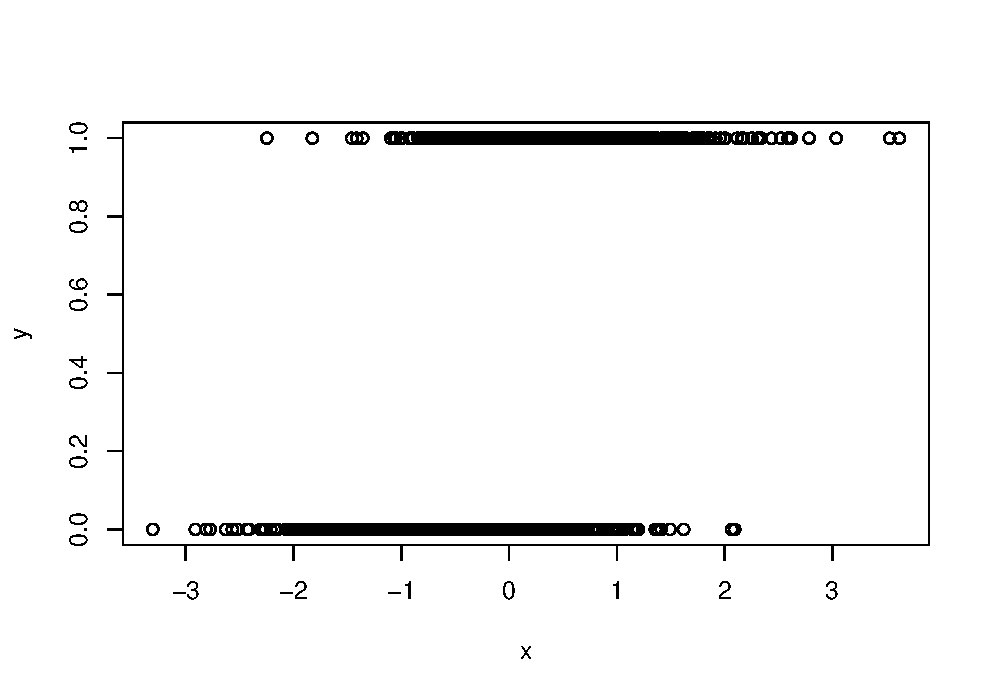
\includegraphics[scale=0.8]{LRS_sample_scatter.pdf}
\end{figure}
\vspace*{-8ex}

Recall the linear regression model:
\[
Y = \alpha + \beta X + e \text{\quad where\quad} e\sim N(0,\sigma^2).
\]
If $Y$ is a binary variable, we cannot apply simple linear regression directly.
\bit
\it OLS regression assumes that $Y\sim N\big(\mu(x),\sigma^2\big)$ where $\mu(x) = \expe(Y|X=x)$.
\it This cannot be true for binary variables.
%\it We want to estimate the conditional probability $p(x) = \prob(Y=1|X=x)$. 
%\it Note that, since $Y\sim\text{Bernoulli}(p(x))$, $p(x)=\expe(Y|X=x)$.
\it A linear model such as $p(x)=\alpha+\beta(x)$ is not appropriate for modelling probabilities.
\eit



%\vspace*{2ex}
%\vspace*{-8ex}
%\begin{figure}[ht]
%\centering
%\caption{Scatter plot for 1000 sample points}
\begin{center}
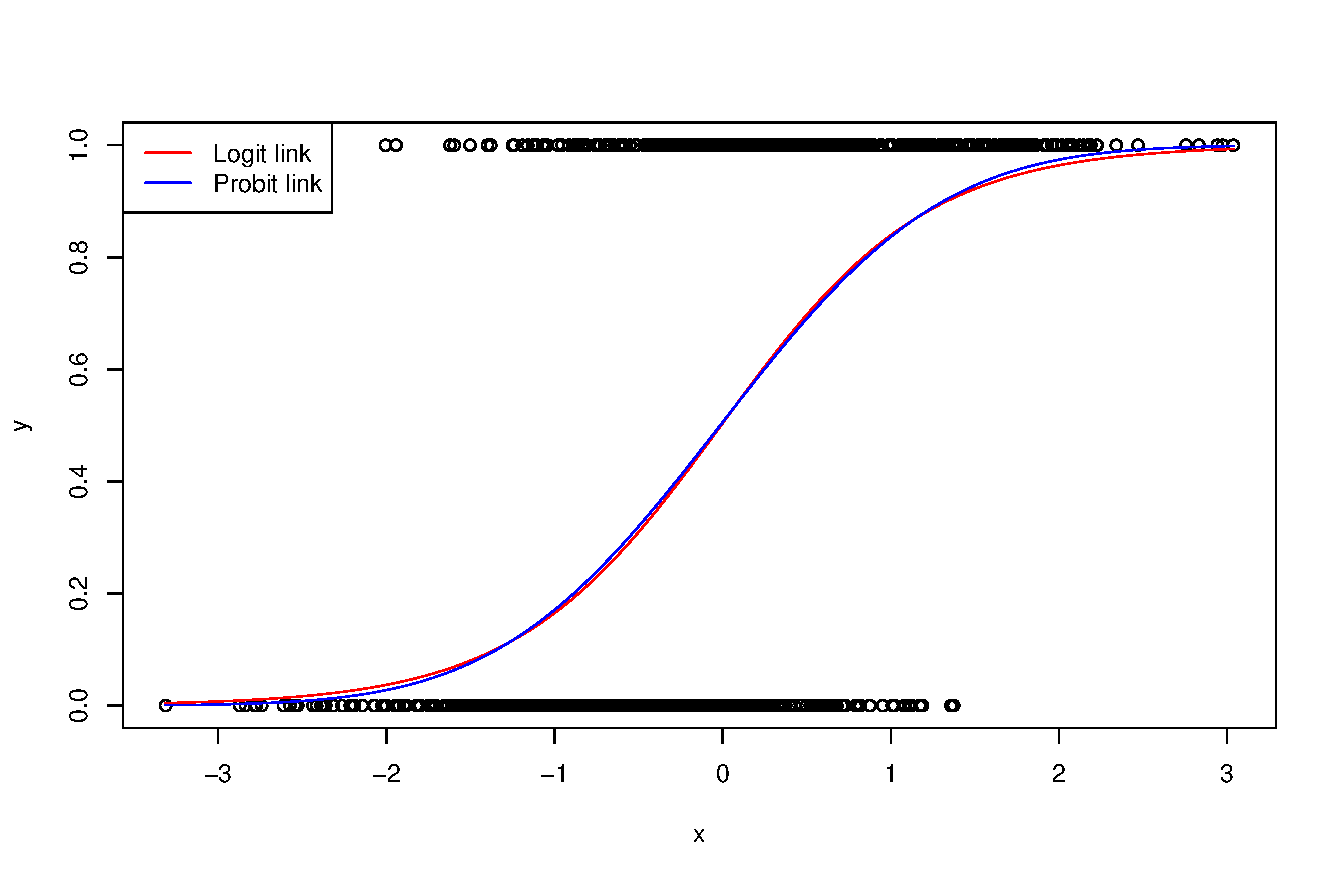
\includegraphics[scale=0.6]{LRS_sample_links.pdf}
\end{center}
%\end{figure}
\vspace*{-2ex}
%\flushall

Under fairly broad conditions, it turns out that the logit function
\[
z(x) = \log\left(\frac{p(x)}{1-p(x)}\right)
\]
is approx.\ normally distributed and approx.\ linearly related to the explanatory variable.
%is approximately (1) normally distributed and (2) linearly related to the explanatory variable(s).

%\bit
%\it is approximately normally distributed, and
%\it is approximately linearly related to the explanatory variable(s).
%\eit 
\bit
\it This is also true of the \emph{probit} function $z(x)=\Phi^{-1}\big[p(x)\big]$.
\it The logit and probit functions are examples of what are called \emph{link functions}.
\it These \emph{link} a probability $p(x)$ with a regression function such as $\alpha+\beta x$.
\eit


Thus we construct a linear model of the logit function $z(x)$ against $x$.
\bit
\it The \emph{null} model: $z(x) = \alpha + e$.
\it The \emph{full} model: $z(x) = \alpha + \beta x + e$.
\eit
%The null hypothesis $H_0:\beta=0$ can be tested using a \emph{log-likelihood} statistic (see later).

\vspace*{2ex}
Having obtained an estimator 
\[
\hat{z}(x) = \hat{\alpha}+\hat{\beta}x,
\]
we can obtain estimates of the probabilities by applying the logistic function:
%Logits are be easily converted back to probabilities:
\[
\hat{p}(x) = \frac{e^{\hat{z}(x)}}{e^{\hat{z}(x)}+1} 
%z = \log\left(\frac{p}{1-p}\right) \quad \Leftrightarrow\quad p = \frac{1}{1+e^{z}} 
%z(x) = \log\left(\frac{p(x)}{1-p(x)}\right) \quad \Leftrightarrow\quad p(x) = \frac{1}{1+\exp(z(x))} 
\]

\bit
%\it The logistic function is the inverse of the logit function.
\it $\hat{p}(x)$ is our model for the conditional probability $p(x)=\prob(Y=1|X=x)$.
\it The null hypothesis $H_0:\beta=0$ can be tested using a \emph{log-likelihood} statistic.
\eit
%Alternatively, 
%\bit
%\it Null model: $\hat{p}(x) = \displaystyle\frac{1}{1+e^{-\alpha}}$.
%\it Full model: $\hat{p}(x) = \displaystyle\frac{1}{1+e^{-(\alpha + \beta x)}}$.
%\eit



%\begin{example}
%%A scientific study looked a 92 male patients who initially survived a first heart attack. 
%\end{example}
%
%Can we estimate the probability that an individual in a population posesses some characteristic, based on the observed value of another characteristic?
%
%\bit
%\it Example 1
%\it Example 2
%\eit
%
%\bit
%%\it $Y$ indicates the presence or absence of a certain characteristic.
%\it Let $A$ be the event that the characteristic is present.
%\it Let $Y$ be the indicator variable of event $A$.
%\eit

%Suppose that $Y$ is the indicator function of some event $A$
%%\vspace*{2ex}
%%Let $Y$ be the indicator variable of event $A$.
%\[
%Y = \left\{\begin{array}{ll}0 & \text{if $A$ does not occur,} \\ 1 & \text{if $A$ occurs.}\end{array}\right. 
%\]
%Then $Y\sim\text{Bernoulli}(p)$ where $p=\prob(A)$.
%
%If we know that $X$ takes the value $x$, can we predict the value of $Y$?
%\bit
%\it Linear regrssion: we estimate the conditional expectation $\expe(Y|X=x) = \alpha + \beta x$.
%\it Logistic regression: we wish to estimate the probability 
%\begin{align*}
%p(x) 
%	& = \prob(Y=1|X=x) \\
%	& = \expe(Y|X=x) \text{\quad because $Y\sim\text{Bernoulli}(p)$}.
%\end{align*}
%\it A linear model $p(x) = \alpha + \beta x$ is not appropriate.
%\eit
%
%Logistic model:
%\[
%p(x) = \frac{1}{1+e^z(x)} \quad \Leftrightarrow\quad z(x) = \log\left(\frac{p(x)}{1-p(x)}\right)
%\]

%\bit
%\it Since $\expe(Y|X=x)\in [0,1]$, the linear model $Y=\alpha+\beta x + e$ is not appropriate.
%\it Instead, we consider the \emph{logistic} transformation of $Y$:
%\eit
%
%Let $\pi=\prob(A)=\prob(Y=1)$.

%====================================================================

\subsection{Conditions}
%====================================================================
\vspace*{2ex}
To apply binary logistic regression, we require that 
\bit
\it The output variable is binary.
\it The observations are independent.
\it The two output categories are mutually exclusive and exhaustive.
\eit

\vspace*{2ex}
We do \emph{not} require that
\bit
\it the output variable is normally distributed, nor that
\it there is a linear relationship between $X$ and $Y$, nor that
\it the variance is constant across different values of $X$.
\eit

%
%
%\underline{Binary logistic regression}. To estimate $p(x) = \prob(Y=1|X=x)$, %= \expe(Y|X=x).
%\ben
%\it 
%Apply the logit function to compute the log-odds for $p(x)$, % in $[0,1]$ to the sol-called log-odds in $[-\infty,+\infty]$:
%\[
%z(x) = \log\left(\frac{p(x)}{1-p(x)}\right)
%\]
%\it
%%
%%Logistic model. 
%%\begin{align*}
%%p = \frac{1}{1+e^{-z}}
%%	& \Rightarrow p(1+e^{-z}) = 1 \\
%%	& \Rightarrow e^{-z}) = \frac{1-p}{p} \\
%%	& \Rightarrow z = \log\left(\frac{p}{1-p}\right)
%%\end{align*}
%Find maximum likelihood estimates $\hat{\alpha}$ and $\hat{\beta}$ for the parameters of the linear model
%\[
%z = \alpha + \beta x + e \text{\quad where\quad} e\sim N(0,\sigma^2).
%\]
%%
%%The coefficients $\alpha$ and $\beta$ are estimated using ordinary least-squares.
%\it
%Apply the logistic function to $\hat{z}=\hat{\alpha}+\hat{\beta}x$ to obtain an estimate of $p(x)$,
%\[
%\hat{p}(x) = \frac{\exp(\hat{\alpha} + \hat{\beta} x)}{1+\exp(\hat{\alpha}+\hat{\beta} x)}
%\]
%\[
%\hat{p}(x) = \frac{e^{\hat{\alpha}+\hat{\beta} x}}{1+e^{\hat{\alpha}+\hat{\beta} x}}.
%\]
%\een
%

%====================================================================

\section{Odds and log-odds}
%====================================================================
The \emph{odds} for an event $A$ are defined by
\[
\odds(A) = \frac{\prob(A)}{1-\prob(A)}.% = \frac{\pi}{1-\pi}.
\]

\vspace*{2ex}
Example: if $\prob(A)=1/4$ then $\odds(A)=1/3$, and we say that
\bit 
\it the odds \emph{for} event $A$ are \emph{one-to-three}, or alternatively,
\it the odds \emph{against} event $A$ are \emph{three-to-one}.
%\it the odds \emph{for} event $A$ are \emph{1:3}, or alternatively,
%\it the odds \emph{against} event $A$ are \emph{3:1}.
\it Note that $0\leq\odds(A) \leq \infty$.
\eit

%\bit
%\it $0\leq\odds(A) \leq \infty$.
%\it $\odds(A)$ is a \emph{likelihood ratio}.
%\eit

The logarithm of the odds is called the \emph{log-odds} for event $A$:
\[
\logodds(A) = \log\left(\frac{\prob(A)}{1-\prob(A)}\right).% = \log\left(\frac{\pi}{1-\pi}\right).
\]
%\begin{align*}
%\logit(A) 
%	& = \log\left(\frac{\prob(A)}{1-\prob(A)}\right) \\
%	& = \log\prob(A) - \log(1-\prob(A)).
%\end{align*}
\bit
\it Note that $-\infty\leq\logodds(A)\leq\infty$.
\eit



The logit function transforms probabilities to log-odds:
\[
\begin{array}{lclc}
\logit:	& [0,1]	& \to 		& \R \\ 
		& p 	& \mapsto	& \log\displaystyle\left(\frac{p}{1-p}\right) 
%		& p 	& \mapsto	& \log\displaystyle\frac{p}{1-p}
\end{array}
%	= \log p - \log(1-p).
\]
This is the inverse of the logistic function.
%Let $\pi = \prob(A)$.
%
%We perform linear regression of $\logit$ against $X$:
%\[
%\logit = \alpha + \beta x
%\]

%Table 1. The relationship between probability of success (p) and logit(p)
\[
\begin{array}{|c|ccccccccc|}\hline
p 				& 0.3		& 0.4		& 0.5	& 0.6	& 0.7	& 0.8	& 0.9	& 0.95	& 0.99 \\
\logit(p)	
%\log\big(\frac{p}{1-p}\big)
%\log\big(p/(1-p)\big)
%\log\left(\frac{p}{1-p}\right)
& -0.847	& -0.405	& 0.000	& 0.405	& 0.847	& 1.386	& 2.197	& 2.944	& 4.595 \\ \hline
\end{array}
\]

Logistic regression involves fitting data to an equation of the form
\[
\log\left(\frac{p(x)}{1-p(x)}\right) = \alpha + \beta x + e.
\]
\bit
\it The logit serves as a \emph{link function} between $p(x)$ and the regression equation $\alpha+\beta x$.
\it Many different link functions are possible (see the \emph{generalized linear model}).
\eit

%This yields the simple \emph{binary logistic model}.
%\[
%\hat{p}(x) = \frac{e^{\hat{\alpha} + \hat{\beta} x}}{1+e^{\hat{\alpha}+\hat{\beta} x}}
%\]
%\[
%\hat{p}(x) = \frac{\exp(\hat{\alpha} + \hat{\beta} x)}{1+\exp(\hat{\alpha}+\hat{\beta} x)}
%\]

%%====================================================================
%
%\section{The logistic function}
%%====================================================================
%The \emph{logistic function} $p:\R\to[0,1]$ is defined by 
%\[
%p(z) =\frac{e^z}{e^z+1} = \frac{1}{1+e^{-z}}	\text{\quad for $z\in\R$.}
%\]
%%This is called the \emph{logistic function}.
%\bit
%\it The value of $p(z)$ can be interpreted as a probability.
%\it $p(z)$ is continuous and strictly increasing.
%\it $\lim_{z\to-\infty}g(z)=0$ and $\lim_{z\to\infty}g(z)=1$.
%\eit
%
%If $z = \alpha + \beta x$ for some explanatory variable $x$, then
%\[
%p(x) 
%%	= \frac{e^{\alpha+\beta x}}{e^{\alpha+\beta x}+1} 
%	= \frac{1}{1+e^{-(\alpha+\beta x)}}.
%\]
%\bit
%\it This is the \emph{simple logistic model}.
%\it The linear model $\alpha+\beta x$ can take any value in $\R$.
%\it The logistic function transforms this to a value between $0$ and $1$.
%\eit
%
%%====================================================================
%\subsection{The logit function}
%%====================================================================
%The inverse of the logistic function is called the \emph{logit function}:
%\[
%\logit(x) = \log\left(\frac{p(x)}{1-p(x)}\right) = \alpha + \beta x
%\]
%
%\bit
%\it The logit serves as a \emph{link function} between $p(x)$ and the regression equation $\alpha+\beta x$.
%\it Many different link functions are possible under the \emph{generalized linear model}.
%\eit
%
%This is the simple \emph{binary logistic model}.
%\[
%\hat{p}(x) = \frac{e^{\hat{\alpha} + \hat{\beta} x}}{1+e^{\hat{\alpha}+\hat{\beta} x}}
%\]
%\[
%\hat{p}(x) = \frac{\exp(\hat{\alpha} + \hat{\beta} x)}{1+\exp(\hat{\alpha}+\hat{\beta} x)}
%\]

%%----------
%\begin{figure}
%\includegraphics[width=0.90\textwidth]{logistic}\\
%\caption{Logistic function}
%\end{figure}
%%----------

%
%\underline{Logistic regression}. To estimate $p(x) = \prob(Y=1|X=x)$, %= \expe(Y|X=x).
%\ben
%\it 
%Apply the logit function to compute the log-odds for $p(x)$, % in $[0,1]$ to the sol-called log-odds in $[-\infty,+\infty]$:
%\[
%z(x) = \log\left(\frac{p(x)}{1-p(x)}\right)
%\]
%\it
%%
%%Logistic model. 
%%\begin{align*}
%%p = \frac{1}{1+e^{-z}}
%%	& \Rightarrow p(1+e^{-z}) = 1 \\
%%	& \Rightarrow e^{-z}) = \frac{1-p}{p} \\
%%	& \Rightarrow z = \log\left(\frac{p}{1-p}\right)
%%\end{align*}
%Find maximum likelihood estimates $\hat{\alpha}$ and $\hat{\beta}$ for the parameters of the linear model
%\[
%z = \alpha + \beta x + e \text{\quad where\quad} e\sim N(0,\sigma^2).
%\]
%%
%%The coefficients $\alpha$ and $\beta$ are estimated using ordinary least-squares.
%\it
%Apply the logistic function to $\hat{z}=\hat{\alpha}+\hat{\beta}x$ to obtain an estimate of $p(x)$,
%\[
%\hat{p}(x) = \frac{\exp(\hat{\alpha} + \hat{\beta} x)}{1+\exp(\hat{\alpha}+\hat{\beta} x)}
%\]
%\een
%====================================================================

\section{Parameter estimation}
%====================================================================
%Instead of using a least-squared deviations criterion for the best fit, it uses a maximum likelihood method, which maximises the probability of getting the observed results given the fitted regression coefficients. 
%
%A consequence of this is that the goodness of fit and overall significance statistics used in logistic regression are different from those used in linear regression.

%\underline{Goal}: 
We want to model the conditional probability $p(x) = \prob(Y=1|X=x)$ as a function of $x$.

%Let
%\[
%p(x) = \prob(Y=1|X=x).
%\]
%

%Can we use linear regression to solve this?
%\bit
%\it $p(x) = \alpha + \beta x$? No - $p(x)$ is restricted to $[0,1]$.
%\it $\log p(x) = \alpha + \beta x$? No - $\log p(x)$ is restricted to $[0,\infty)$.
%\it $\log\big[p(x)/(1-p(x))\big]$? OK.
%\eit

\vspace*{2ex}
The \emph{logistic regression} model is
%\[
%p(x) = \frac{1}{1+e^{-(\alpha+\beta x + e)}}\text{\quad where\quad} e\sim N(0,\sigma^2).
%\]
%
%This can be written as
\[
\log\left(\frac{p(x)}{1-p(x)}\right) = \alpha + \beta x + e \text{\quad where\quad} e\sim N(0,\sigma^2).
\]
%\bit
%\it The LHS is called the \emph{logit} of $p(x)$.
%\it It can be modelled against $x$ using OLS regression.
%\eit
%

Let $\{(X_1,Y_1),(X_2,Y_2),\ldots,(X_n,Y_n)\}$ be a random sample.

\bit
\it If $X_i=x_i$ then $Y_i\sim\text{Bernoulli}\big(p(x_i)\big)$.%where $p(x_i)=\prob(Y=1|X=x_i)$.
\it In this case, $\expe(Y_i) = p(x_i)$ and $\var(Y_i) = p(x_i)\big(1-p(x_i)\big)$.
\it If $\beta\neq 0$, the $Y_i$ are not identically distributed.
\eit
%Let $(x_1,y_1),(x_2,y_2),\ldots,(x_n,y_n)$ be a realization of the sample. 
The likelihood function is
\[
%L(\alpha,\beta;\mathbf{x},\mathbf{y}) = \prod_{i=1}^n  p(x_i)^{y_i}\big(1-p(x_i)\big)^{1-y_i}.
L(\alpha,\beta) = \prod_{i=1}^n  p(x_i)^{y_i}\big(1-p(x_i)\big)^{1-y_i}.
\]
The log-likelihood function is
\[
\ell(\alpha,\beta) = \sum_{i=1}^n \big[y_i\log p(x_i) + (1-y_i)\log(1-p(x_i))\big].
\]
Substituting for $p(x_i) = 1/(1+e^{-(\alpha+\beta x_i)})$, we obtain
\[
\ell(\alpha,\beta) = \sum_{i=1}^n \big[y_i(\alpha+\beta x_i) - \log(1+e^{\alpha+\beta x_i})\big].
\]
To find the MLEs of $\alpha$ and $\beta$, we must solve
\[
\frac{\partial\ell(\alpha,\beta)}{\partial\alpha} = 0 \text{\quad and\quad} \frac{\partial\ell(\alpha,\beta)}{\partial\beta} = 0.
\]
\bit
\it These yield two equations that are \emph{non-linear} in $\alpha$ and $\beta$.
\it In most cases, they must be solved numerically (e.g.\ using the Netwon-Rhapson method).
\eit

%It turns out that $2\ell \sim X^2_1$.
%====================================================================

\section{Model evaluation}
%====================================================================

%Recall that $p(x)=\prob(Y=1|X=x)$, and also the log-likelihood function:
The log-likelihood function is
\[
\ell(\alpha,\beta) =\sum_{i=1}^n\left[y_{i}\log p(x_i) +(1-y_i)\log(1-p(x_i))\right]
\text{\quad where\quad}
p(x)=\frac{e^{\alpha+\beta x}}{1+e^{\alpha+\beta x}}.
\]
%where $p(x) = \exp(\alpha+\beta x)/(1+\exp(\alpha+\beta x))$.
%
%\vspace*{2ex}
%$p(x)=e^{\alpha+\beta x}/(1+e^{\alpha+\beta x})$.
%
%\bit
%\it Let $\hat{\alpha}$ and $\hat{\beta}$ denote the MLEs of $\alpha$ and $\beta$.
%\eit

\vspace*{2ex}
We can estimate the probabilities $p(x_i)$ by the fitted values $\hat{p}(x_i)\in[0,1]$.
%\bit
%\it We can estimate the $p(x_i)$ by the fitted values $\hat{p}(x_i)\in[0,1]$.
%\it This yields the \emph{empirical} log-likelihood function:
%\eit
%We can estimate this using the estimated probabilities $\hat{\prob}(x_i)$.
\[
\hat{\ell}(\mathbf{x},\mathbf{y}) = \sum_{i=1}^n \big[y_i\log \hat{p}(x_i) + (1-y_i)\log(1-\hat{p}(x_i))\big]
\text{\quad where\quad}
\hat{p}(x)=\frac{e^{\hat{\alpha}+\hat{\beta} x}}{1+e^{\hat{\alpha}+\hat{\beta} x}}.
\]

%\vspace*{2ex}
%We can also replace the $p(x_i)$ by the estimated values $\hat{y}_i\in\{0,1\}$:
%\[
%T(\mathbf{x},\mathbf{y}) = \sum_{i=1}^n \big[y_i\log \hat{p}(x_i) + (1-y_i)\log(1-\hat{p}(x_i))\big]
%\text{\quad where\quad}
%\hat{p}(x)=\frac{e^{\hat{\alpha}+\hat{\beta} x}}{1+e^{\hat{\alpha}+\hat{\beta} x}}.
%\]
%
%\[
%\hat{p}(x) = \frac{\exp(\hat{\alpha} + \hat{\beta} x)}{1+\exp(\hat{\alpha}+\hat{\beta} x)}.
%\]

%
%\[
%\hat{y}_i = \left\{\begin{array}{ll}
%	0	& \text{ when $\hat{p}(x_i)\leq 0.5$}, \\
%	1	& \text{ when $\hat{p}(x_i)>0.5$}.
%\end{array}\right.
%\]
%
%
%
%This yields the \emph{empirical} log-likelihood function,
%\[
%LL = \sum_{i=1}^n \big[y_i\log\hat{y}_i + (1-y_i)\log(1-\hat{y}_i)\big]
%\]

%Distribution?
\bit
%\it It turns out that 
%\it $\hat{\alpha}$ and $\hat{\beta}$ are respectively the MLEs of $\alpha$ and $\beta$.
\it This is analogous to the residual sum of squares in linear regression
\it It quantifies the amount of unexplained variation remaining after the model has been fitted.
\it A large value of the log-likelihood indicates a poor fit.
\eit


The \emph{deviance} of the model is defined to be
\[
D = -2\log\left(\frac{\text{Likelihood of null model}}{\text{Likelihood of full model}}\right)
\]

Under the null hypothesis $H_0:\beta=0$,
\bit
\it It can be shown that $D$ has chi-squared distribution.
\it This can be used to test the significance of $X$ as a predictor of $Y$.
\eit

%====================================================================

\section{Numerical example}
%====================================================================
Consider the data shown in the following table:
\[
\begin{array}{|c|cccccccccc|}\hline
x	& 1 & 2 & 3 & 4 & 5 & 6 & 7 & 8 & 9 & 10 \\ \hline
y	& 0 & 0 & 0 & 0 & 1 & 0 & 1 & 0 & 1 & 1 \\ \hline
\end{array}
\]	

The Newton-Rhapson method is commonly used to obtain numerical estimate $\alpha$ and $\beta$:
\begin{center}
\begin{tabular}{|c|ll|} \hline
Iteration	& Deviance & \\ \hline
1 	& 13.4602 & (Null Model) \\
2 	& 8.9873 & \\
3	& 8.6395 & \\
4	& 8.6203 & \\
5	& 8.6202 & \\
6	& 8.6202 & (Converged) \\ \hline
\end{tabular}
\end{center}



\underline{Parameter estimates}:
\bit
\it Intercept: $\hat{\alpha} = -4.3578$.
%\it $\hat{\beta} = 0.6622$, $\hat{\sigma}_{\hat{\beta}}=0.4001$, $p\text{-value}=0.0979$.
\it Gradient: $\hat{\beta} = 0.6622$ ($p\text{-value}=0.0979$).
%\it Gradient: $\hat{\beta} = 0.6622$, $\text{StdErr}(\hat{\beta})=0.4001$, $p\text{-value}=0.0979$.
%\it Goodness-of-Fit: $\chi^2_1 = 4.8400$, $p\text{-value}=0.0278$.
%\it Odds ratio: $1.9391$. Confidence interval $(0.8852, 4.2478)$
\eit

\vspace*{2ex}
\underline{Goodness-of-fit}:
\bit
%\it Intercept: $\hat{\alpha} = -4.3578$.
%%\it $\hat{\beta} = 0.6622$, $\hat{\sigma}_{\hat{\beta}}=0.4001$, $p\text{-value}=0.0979$.
%\it Gradient: $\hat{\beta} = 0.6622$, $\text{StdErr}(\hat{\beta})=0.4001$, $p\text{-value}=0.0979$.
\it Chi-squared statistic: $\chi^2_1 = 4.8400$ ($p\text{-value}=0.0278$).
%\it Odds ratio: $1.9391$. Confidence interval $(0.8852, 4.2478)$
\eit

\vspace*{2ex}
\underline{Model}:
\[
\log\left(\frac{\hat{p}(x)}{1-\hat{p}(x)}\right) = -4.3578 + 0.6622 x,
\]
or equivalently,
\[
\hat{p}(x) = \frac{1}{1+\exp(4.3578 - 0.6622 x)}.
\]

\vspace*{2ex}
\underline{Prediction rule}:
\[
\hat{Y}_i = \left\{\begin{array}{ll}
	0	& \text{ when $\hat{p}(x_i)\leq 0.5$}, \\
	1	& \text{ when $\hat{p}(x_i)>0.5$}.
\end{array}\right.
\]

\vspace*{2ex}

The estimated probabilities $\hat{p}(x_i)$ shown in the following table:
\[
\begin{array}{|c|cccccccccc|}\hline
x			& 1 & 2 & 3 & 4 & 5 & 6 & 7 & 8 & 9 & 10 \\ \hline
y			& 0 & 0 & 0 & 0 & 1 & 0 & 1 & 0 & 1 & 1 \\  \hline\hline
\hat{p}(x)	& 0.024 & 0.046 & 0.085 & 0.153 & 0.260 & 0.405 & 0.569 & 0.719 & 0.832 & 0.906 \\ \hline
\hat{y}		& 0 & 0 & 0 & 0 & 0 & 0 & 1 & 1 & 1 & 1 \\  \hline
|y-\hat{y}|	& 0 & 0 & 0 & 0 & 1 & 0 & 0 & 1 & 0 & 0 \\  \hline
\end{array}
\]	

The model can be assessed in a number of different ways:
\bit
\it False positive rate: $1/10$ (case $x=8$).
\it False negative rate: $1/10$ (case $x=5$).
\it Gini coefficient.
\it And so on ...
\eit

%%====================================================================
%\section{Comparing models}
%%====================================================================
%Calculate a log-likelihood for different models and to compare these models by looking at the difference between their log-likelihoods.
%\[
%\chi^{2}=2\left[\ell(new)-\ell(baseline)\right]
%\]
%and $df=k_{new}-k_{baseline}$
%
%%====================================================================
%\section{Assessing predictors: The Wald statistic}
%%====================================================================
%\[
%Wald=\frac{b}{SE[b]}
%\]
%
%\bit
%\it Similar to t-statistic in usual regression
%\it Tests the null hypothesis that $b = 0$
%\it Is biased when $b$ is large
%\eit

%%====================================================================
%\section{Assessing predictors: The odds ratio or $\exp{(b)}$}
%%====================================================================
%The \emph{odds-ratio} is 
%\[
%\exp{(b)}=\frac{\textrm{Odds after a unit change in predictor}}{\textrm{Odds before a unit change in predictor}}
%\]
%
%\bit
%\it $\frac{\pi}{1-\pi}$ is known as an odds ratio
%\it Indicates the change in odds resulting from a unit change in the predictor
%\it $OR>1$:Predictor $\uparrow$, Probability of outcome occurring $\uparrow$
%\it $OR<1$:Predictor $\uparrow$, Probability of outcome occurring $\downarrow$
%\eit

%======================================================================
\stopcontents[chapters]
\endinput
%====================================================================
